\section{Description of the Project}
Figure~\ref{fig:cluster_network} shows the output of our visualization. 

\begin{figure}[htb]
 \centering
     {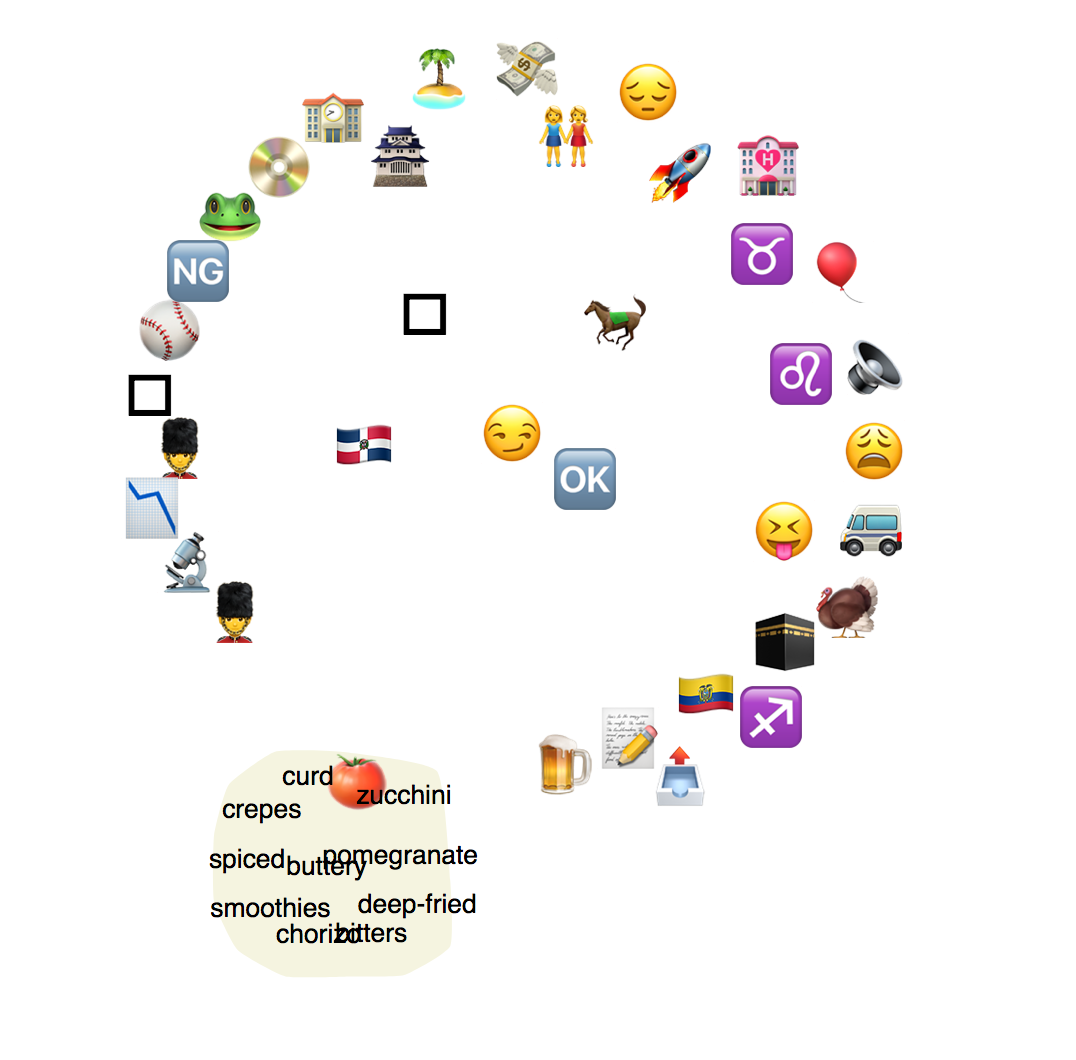
\includegraphics[width=0.58\linewidth]{clustered_network.png}}
    \vspace{-1ex}
     \caption{The visualizaiton of word embeddings using clustered network and emojis.}
\label{fig:cluster_network}
\end{figure}


Our approach for constructing the visualization is as follows:
\begin{enumerate}
 \item Train a word embedding
 \item Run k-means and obtain clusters
 \item Assign an emoji to each cluster
 \item Visualize using D3.js
\end{enumerate}

\subsection{Annotation of Clusters with Emojis}
When a human look at emoji, one connects with various possible concepts. 
Searching for a right word to represent the cluster requires external linguistic resources e.g., WordNet. 
However, images does not associate a single word. 
For example, when one looks at 🍅, the possible association of this words are ``tomato'', ``vegatable'', ``food'', or even ``object''. 
Therefore, we decide to use emojis to represent the clusters. 


\subsection{Interaction}
Users can click on emojis to ``drill-down'' \cite{Elmqvist:2010:HAI:1749404.1749525} the cluster and look into which words are in the cluster.


\subsection{Force Layout}
To solve the problem of overlapping texts, we also use force layout in D3.js to let the texts and emojis move and draggable. 
